This test case represents a scenario in which different objects are born at different times and move in various directions. It demonstrates how well the filter performs on tracking multiple objects when the number of true targets $X_k$ changes over time.

The birth intensity consists of two Gaussian terms, as in the (C1) case, each with a weight of $0.1$, and is expressed as follows:

\begin{equation}\label{eq:c2-birth}
    \gamma_k(\mathbf{x}) = 0.1 \mathscr{N}\left( \mathbf{x}; \svecat{m}{\gamma}{(1)}, \vecat{P}{\gamma} \right)
        + 0.1 \mathscr{N}\left( \mathbf{x}; \svecat{m}{\gamma}{(2)}, \vecat{P}{\gamma} \right),
\end{equation}

\noindent where:

\begin{equation}\label{eq:c2-birth-means}
    \svecat{m}{\gamma}{(1)} = \begin{bmatrix}
        -1000 \\
        750 \\
        0 \\
        0 \\
    \end{bmatrix},
    \qquad
    \svecat{m}{\gamma}{(2)} = \begin{bmatrix}
        1000 \\
        -750 \\
        0 \\
        0 \\
    \end{bmatrix},
    \qquad
    \vecat{P}{\gamma} = \begin{bmatrix}
        100 & 0     & 0     & 0     \\
        0   & 100   & 0     & 0     \\
        0   & 0     & 30    & 0     \\
        0   & 0     & 0     & 30    \\
    \end{bmatrix}.
\end{equation}

In total, there are six different tracks, with a maximum of five targets present at a time and a minimum of one target at a time step. Objects are born every $10$ time steps, and each has a lifespan of $50$ time steps. The paths of the six targets are depicted in Figure \ref{fig:c2-scenario}. The state vectors of the six targets are as follows:

\begin{alignat}{3}\label{eq:c2-init-states}
    \svecat{x}{0}{(1)} &= \begin{bmatrix}
        -1000.0 \\
        750.0 \\
        25.0 \\
        0.0
    \end{bmatrix},
    &\qquad
    \svecat{x}{10}{(2)} &= \begin{bmatrix}
        1000.0 \\
        -750.0 \\
        -25.0 \\
        0.0
    \end{bmatrix},
    &\qquad
    \svecat{x}{20}{(3)} &= \begin{bmatrix}
        -1000.0 \\
        750.0 \\
        17.68 \\
        -17.68
    \end{bmatrix},
    \nonumber \\
    \svecat{x}{30}{(4)} &= \begin{bmatrix}
        1000.0 \\
        -750.0 \\
        -17.68 \\
        17.68
    \end{bmatrix},
    &\qquad
    \svecat{x}{40}{(5)} &= \begin{bmatrix}
        -1000.0 \\
        750.0 \\
        0.0 \\
        -25.0
    \end{bmatrix},
    &\qquad
    \svecat{x}{50}{(6)} &= \begin{bmatrix}
        1000.0 \\
        -750.0 \\
        0.0 \\
        25.0
    \end{bmatrix}.
\end{alignat}

\begin{figure*}
    \centering
    \begin{subfigure}[]{0.48\linewidth}
        \centering
        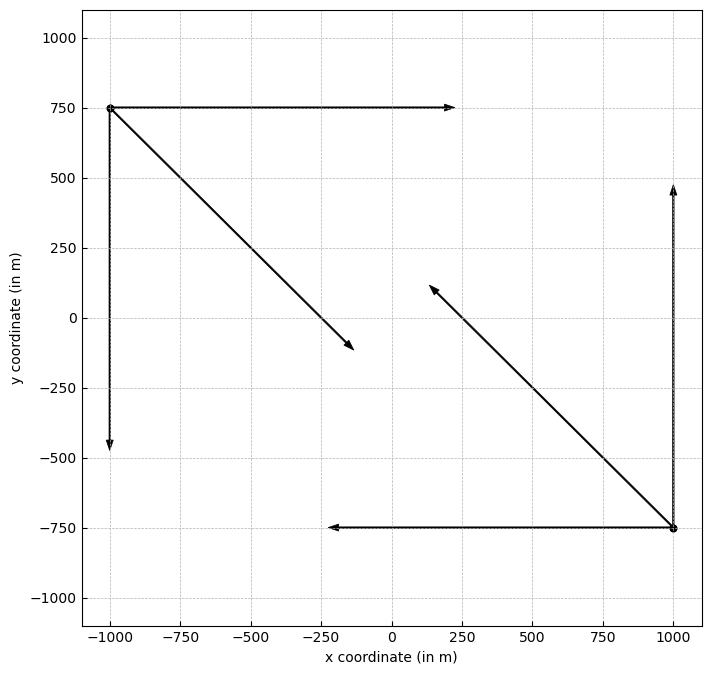
\includegraphics[width=\linewidth]{figures/c2-tracks.png}
    \end{subfigure}
    \hfill
    \begin{subfigure}[]{0.48\linewidth}
        \centering
        \begin{subfigure}[t]{\linewidth}
            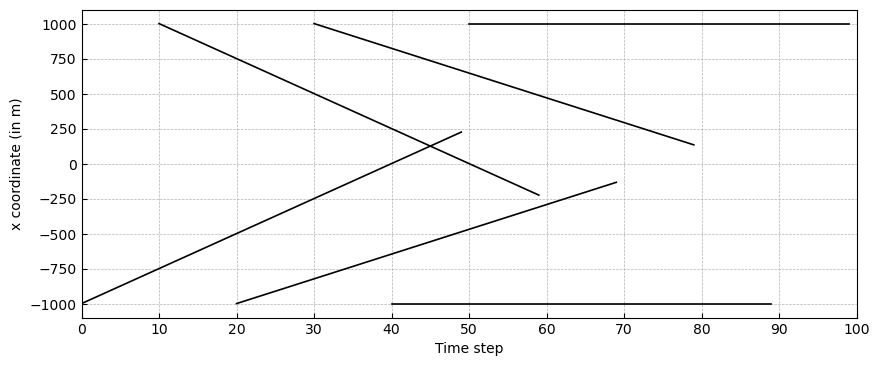
\includegraphics[width=\linewidth]{figures/c2-coord-x.png}
        \end{subfigure}
        \vfill\par
        \begin{subfigure}[b]{\linewidth}
            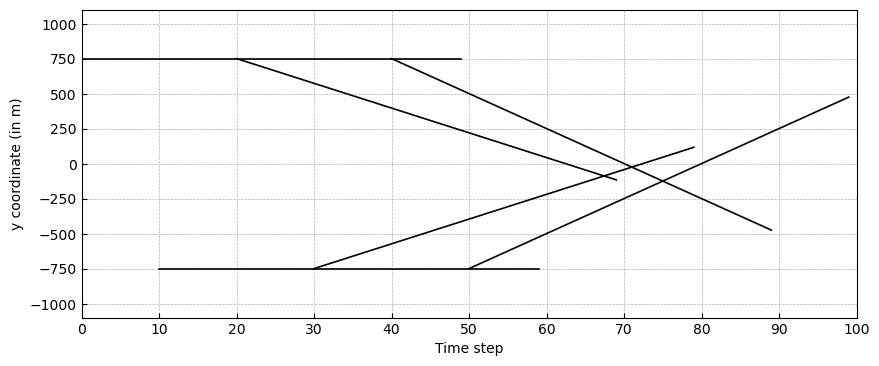
\includegraphics[width=\linewidth]{figures/c2-coord-y.png}
        \end{subfigure}
    \end{subfigure}
  \caption[True tracks of objects in the (C2) scenario.]{The (C2) scenario. In the left figure, we can see the tracks of multiple objects in the 2D space, their locations of birth (black circles) and death (arrow heads). The right figure shows how the coordinates of each object track change over time and the variation in the number of objects present in the scene.}
  \label{fig:c2-scenario}
\end{figure*}
